\documentclass[11pt]{article}
\usepackage{graphicx}
\usepackage{hyperref}
\usepackage{natbib}
\usepackage{amsmath}

\setlength{\textwidth}{6.5in}
\setlength{\headheight}{0in}
\setlength{\textheight}{8.0in}
\setlength{\hoffset}{0in}
\setlength{\voffset}{0in}
\setlength{\oddsidemargin}{0in}
\setlength{\evensidemargin}{0in}

\title{PS4}
  
\author{Shihong Pan\\ \url{https://github.com/PSH-hub24/phys-ga2000}}


\begin{document}

\maketitle

\section{Q1}
Fig \ref{fig:Q1b} shows the heat capacity from 5K to 500K. Fig \ref{fig:Q1c} shows the plot with different choices of $N$. But the curves mostly overlap with each other even after decreasing the linewidth, so it is hard to tell the difference.

\section{Q2}
Since $E=V(a)$, rearranging we have
\begin{equation}
    \frac{dx}{dt}=\sqrt{\frac{2(V(a)-V(x))}{m}}.
\end{equation}
Separate $dx$ and $dt$, then integrate over a quarter of the period $T$ (0 to $T/4$ w.r.t $t$, 0 to $a$ w.r.t $x$), we have
\begin{equation}
    \frac{T}{4}=\int^a_0\sqrt{\frac{m}{2(V(a)-V(x))}}dx
\end{equation}
which give
\begin{equation}
    T = \sqrt{8m}\int^a_0\frac{dx}{\sqrt{V(a)-V(x)}}.
\end{equation}
Fig \ref{fig:Q2b} shows the plot of period for part b. The result makes sense because the potential is $V(x)=x^4$. It leaves some order of $x$ in the denominator of the definite integral of $x$, which gives a inversely proportional relationship between $T$ and amplitude.

\section{Q3}
Fig \ref{fig:Q3a} shows the wavefunctions for $n=0,1,2,3$. Fig \ref{fig:Q3b} plots $n=30$. Fig \ref{fig:Q3cd} calculates the rms position for part c and part d.

\begin{figure}[b!]
\centering
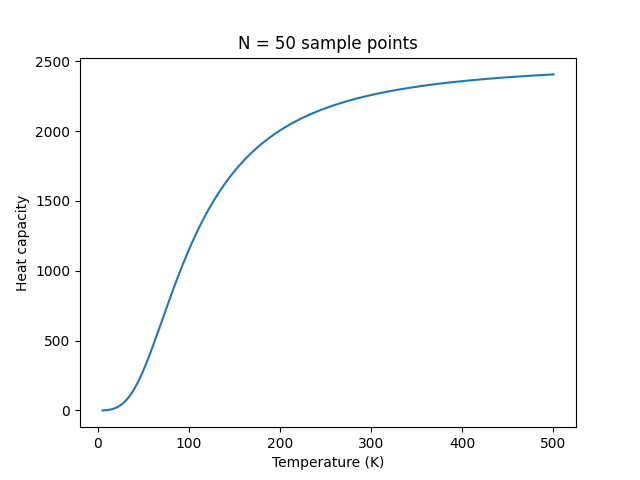
\includegraphics[width=0.6\textwidth]{Computational Physics/ps4Figures/q1(N=50).png}
\caption{The plot for Q1 part b.}
  \label{fig:Q1b}
\end{figure}

\begin{figure}[b!]
\centering
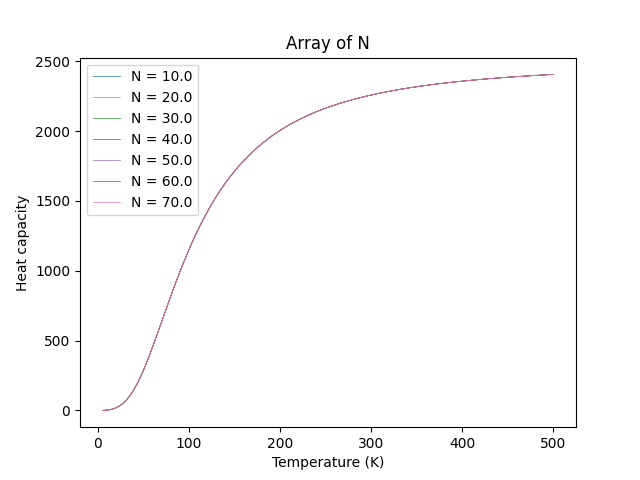
\includegraphics[width=0.6\textwidth]{Computational Physics/ps4Figures/q1(part c).png}
\caption{Q1 part c, different choices of $N$.}
  \label{fig:Q1c}
\end{figure}

\begin{figure}[b!]
\centering
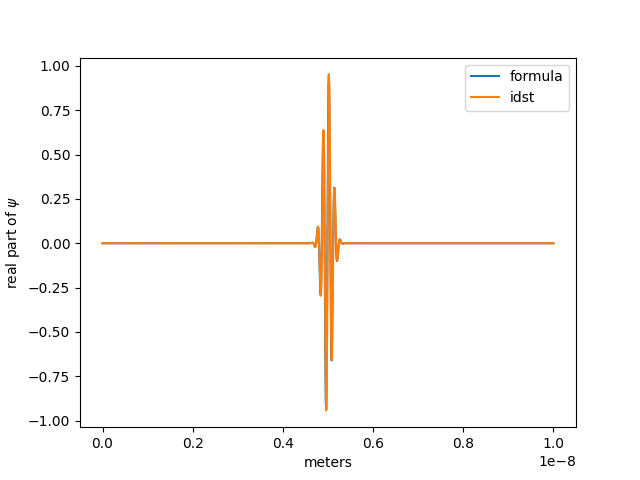
\includegraphics[width=0.6\textwidth]{Computational Physics/ps4Figures/q2b.png}
\caption{Q2 part b, the period for amplitudes ranging from 0 to 2.}
  \label{fig:Q2b}
\end{figure}

\begin{figure}[b!]
\centering
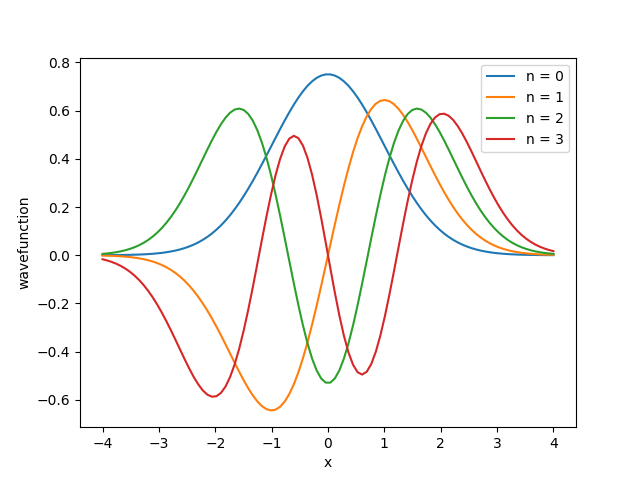
\includegraphics[width=0.6\textwidth]{Computational Physics/ps4Figures/q3a.png}
\caption{Q3 part a, the wavefunctions for $n=0,1,2,3$.}
  \label{fig:Q3a}
\end{figure}

\begin{figure}[b!]
\centering
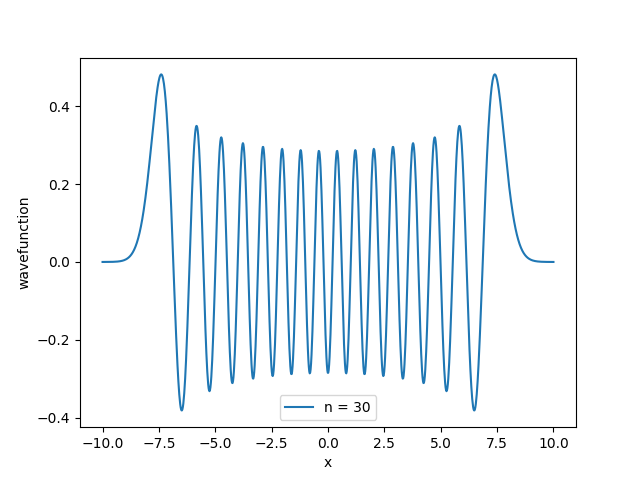
\includegraphics[width=0.6\textwidth]{Computational Physics/ps4Figures/q3b.png}
\caption{Q3 part b, $n=30$.}
  \label{fig:Q3b}
\end{figure}

\begin{figure}[b!]
\centering
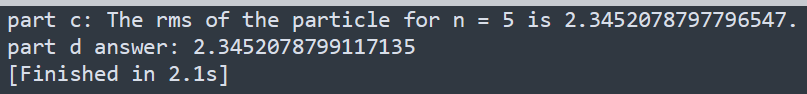
\includegraphics[width=0.6\textwidth]{Computational Physics/ps4Figures/q3cd.PNG}
\caption{Q3 part c and d, the rms position calculated using the previous program (part c) and Gauss-Hermite quadrature (part d).}
  \label{fig:Q3cd}
\end{figure}

\bibliographystyle{apj}
\bibliography{example}

\end{document}

 
 
